\documentclass[12pt,a4paper]{article}
\usepackage{fullpage}
\usepackage[USenglish]{babel}
\usepackage{authblk}
\usepackage{hyperref}
\usepackage{graphicx}
\usepackage{listings}
\usepackage{xcolor}
\usepackage{hyperref}
\usepackage{tabularx}
\usepackage{ragged2e}

\colorlet{punct}{red!60!black}
\definecolor{background}{HTML}{EEEEEE}
\definecolor{delim}{RGB}{20,105,176}
\colorlet{numb}{magenta!60!black}

\lstdefinelanguage{json}{
    basicstyle=\normalfont\ttfamily,
    numbers=left,
    numberstyle=\scriptsize,
    stepnumber=1,
    numbersep=8pt,
    showstringspaces=false,
    breaklines=true,
    frame=lines,
    backgroundcolor=\color{background},
    literate=
     *{0}{{{\color{numb}0}}}{1}
      {1}{{{\color{numb}1}}}{1}
      {2}{{{\color{numb}2}}}{1}
      {3}{{{\color{numb}3}}}{1}
      {4}{{{\color{numb}4}}}{1}
      {5}{{{\color{numb}5}}}{1}
      {6}{{{\color{numb}6}}}{1}
      {7}{{{\color{numb}7}}}{1}
      {8}{{{\color{numb}8}}}{1}
      {9}{{{\color{numb}9}}}{1}
      {:}{{{\color{punct}{:}}}}{1}
      {,}{{{\color{punct}{,}}}}{1}
      {\{}{{{\color{delim}{\{}}}}{1}
      {\}}{{{\color{delim}{\}}}}}{1}
      {[}{{{\color{delim}{[}}}}{1}
      {]}{{{\color{delim}{]}}}}{1},
}

\lstdefinelanguage{tableJson}{
    basicstyle=\small\ttfamily,
    showstringspaces=false,
    breaklines=true,
    aboveskip=0,
    belowskip=0,
    literate=
     *{0}{{{\color{numb}0}}}{1}
      {1}{{{\color{numb}1}}}{1}
      {2}{{{\color{numb}2}}}{1}
      {3}{{{\color{numb}3}}}{1}
      {4}{{{\color{numb}4}}}{1}
      {5}{{{\color{numb}5}}}{1}
      {6}{{{\color{numb}6}}}{1}
      {7}{{{\color{numb}7}}}{1}
      {8}{{{\color{numb}8}}}{1}
      {9}{{{\color{numb}9}}}{1}
      {:}{{{\color{punct}{:}}}}{1}
      {,}{{{\color{punct}{,}}}}{1}
      {\{}{{{\color{delim}{\{}}}}{1}
      {\}}{{{\color{delim}{\}}}}}{1}
      {[}{{{\color{delim}{[}}}}{1}
      {]}{{{\color{delim}{]}}}}{1},
}


\usepackage{todonotes}

% Remove section numbering
\setcounter{secnumdepth}{0}
% Remove paragraph indentation
\setlength{\parindent}{0cm}


\title{eBay Search Service}
\author{Isabel Giang}
\author{Maxwell Wenger}
\affil{CSS490 Group Y4}

\date{January 26, 2021}


\begin{document}
\maketitle
\setcounter{tocdepth}{3}
\tableofcontents

% Problem:
% EBay Search has gotten quite slow.  We were able to gain some time by adding
% an index to the Master DB, but we are worried about long term scaling.  We
% need to settle on a design for a SearchServce that would be used to search
% for Auctions by Keyword and/or Category (breadcrumb)

% Deliverables:
% Create a design document that explains how you would solve the search
% problem.  This document will be read by the various engineers in the company
% for evaluation of your approach,so your design needs to be understandable to
% them based on the document.

\pagebreak
\section{Overview}

This document is intended to explain why the eBay Search Service is being created
and a suggested approach to implement the eBay Search Service for the purposes
of being audited for technical feasibility by an engineer.

\vspace{\baselineskip}

This document will explain the following:

\begin{itemize}
    \item the API designs for each eBay Search Service API
    \item details needed for implementation and to assess if this solution is technically viable
    \item changes that must be made to the eBay Master Service to use the eBay Search Service
\end{itemize} 


\subsection{Problem Statement}
In the last few months, eBay users have reported increasingly slow response
times from eBay's website when searching for auctions. Application log analysis
for the eBay Master Service has confirmed that our FindAuctions API for the
eBay Master service takes significantly longer to return a response when we
search for auctions using keywords. It also takes longer to search for a large
number of auctions.
\vspace{\baselineskip}
This is negatively impacting eBay's user experience for existing users and is
hindering the website's chances of being adopted by new users.

% State business problem
\vspace{\baselineskip}

Performing further analysis on the eBay Master service schema shows that the
FindAuctions API must scan the entire table to first find active auctions. Then
it must scan those active auctions to find auctions that have titles with the
keywords we are looking for.

\subsection{Temporary Solution}

As a bandaid solution to temporarily address this problem, we have added an 
AuctionStatus index to the Auction table of the eBay Master Service database.
This allows us to immediately access all active auctions instead of being forced 
to scan the entire Auction table to find active auctions before querying with keywords. 

\vspace{\baselineskip}
This speeds up the FindAuctions API enough to fix the poor user experience
temporarily, but this will not be enough as the company grows. The number of
records in the Auction table, and subsequently, the number of active auctions
will increase at an exponential rate.



\pagebreak
\subsection{Next Steps}
To solve this more permanently, we want to create a separate search service
that will handle searching for auctions by keyword and/or category. 
We will call this new service the eBay Search Service. 

\vspace{\baselineskip} 
The search service will have its own database that can only be changed
by external users via its API.
We will \emph{delegate} the eBay Master Service's searching to this new Search Service, 
which will allow us to only keep information relevant to searching in the Search Service's database. 

\begin{center}
    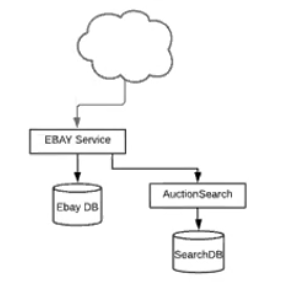
\includegraphics[scale=0.75]{images/new-service.png}
\end{center}

Whenever a new FindAuction API request is made, 
this service will perform the required business logic and databases accesses 
instead of the eBay Master service.

\vspace{\baselineskip}


At a minimum, the eBay Search Service should support searching in the following ways:

\begin{itemize}
    \item Searching for all auctions
    \item Searching for auctions based on auction status (closed, open, pending, cancelled)
    \item Searching for auctions based on keywords
    \item Searching for auctions based on category
    \item Searching for auctions based on keywords and category
\end{itemize}

Each search operation will only allow ``AND'' operations between search terms. 
For example, searching for auctions that have``red'' AND ``yellow'' in their titles.
\vspace{\baselineskip}

``OR'' operations must be done by forming a union of the results from multiple calls. 
For example, to get the results for auctions that have ``red'' OR ``yellow'' in their titles, 
you must combine the results of searching for auctions that have ``red" in their titles,
and the results of searching for auctions that have ``yellow'' in their titles.


\pagebreak
% Clarify what kinds of searching we are doing such as:
% - Allow searching for only active auctions 
% - this one -> Allow searching for any auction.
% - Allow a bidder to find all of their active auctions
% - Administrator looking for a specific set of auctions that have expired
% - Etc

% Need Database Schema
 
\section{eBay Search Service API Specification}

\subsection{API List}
\begin{center}
    \begin{tabular}{| l | l |}
        \hline
        \textbf{API Name} & \textbf{Description} \\
        \hline
            saveSearchableAuction & Updates or creates a searchable auction \\ 
        \hline
            findAuctions & Finds auctions based on the given keywords and/or category. \\
        \hline
    \end{tabular}
\end{center}

\subsection{Schemas}

\subsubsection{SearchDB}
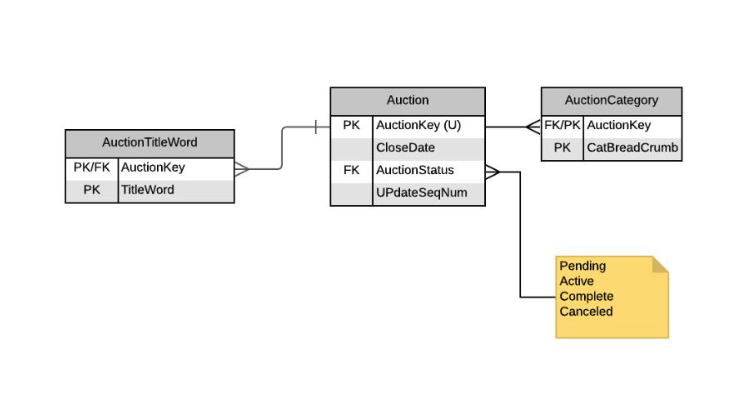
\includegraphics[scale=0.5]{images/search-schema.png}
\subsubsection{MasterDB}
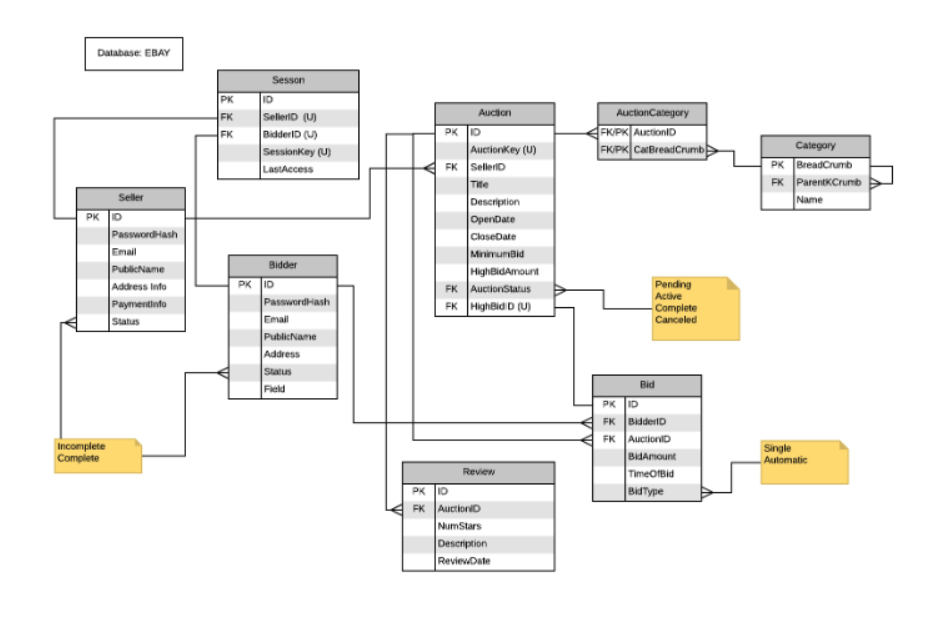
\includegraphics[scale=0.35]{images/master-schema.png}
\pagebreak
\subsection{API Descriptions}

\subsubsection{saveSearchableAuction}
\label{ref:csa}
Creates an auction if no auction that corresponds with the given auction key exists.
Otherwise, updates the auction that corresponds with the given auction key. 

\paragraph{Input}

\begin{itemize}
    \item \textbf{auctionKey} - Public key that uniquely identifies an auction from the eBay Master Service.
    \item \textbf{title} - Title of the auction 
    \item \textbf{closeDate} - Closing date of the auction 
    \item \textbf{categories} -  List of category breadcrumbs
    \item \textbf{status} - Status of the auction (closed, open, pending, cancelled)
    \item \textbf{seqNum} - Sequence number of the auction record. Each time an update is performed for this record,
        it is incremented by one. Requests made with \texttt{seqNum} $<$ \texttt{UpdateSeqNum} for this record are ignored.
\end{itemize}
\begin{lstlisting}[language=json,numbers=none]
{
    "auctionKey": <string>,
    "title": <string>,
    "closeDate": <string>,
    "categories": [ <string>, ...],
    "status": <string>,
    "seqNum": <int>
}
\end{lstlisting}

\paragraph{Output}
\begin{center}
    \begin{tabular}{| p{6cm} | l |}
        \hline
        \textbf{Scenario} & \textbf{Response} \\
        \hline
        Successfully stored an auction & 
        \begin{lstlisting}[language=tableJson,firstnumber=1]
{
    "success": true,
    "seqNum": <int>           
}

        \end{lstlisting} \\ 
        \hline
        Auction key does not match with an existing auction & 
        \begin{lstlisting}[language=tableJson,firstnumber=1]
{
    "success": false,
    "error": "InvalidAuction"
}

        \end{lstlisting} \\ 
        \hline
        \texttt{SeqNum} $<$ \texttt{UpdateSeqNum} for this auction. & 
        \begin{lstlisting}[language=tableJson,firstnumber=1]
{
    "success": false,
    "error": "OutOfOrder"
}

        \end{lstlisting} \\ 
        \hline
    \end{tabular}
\end{center}



\pagebreak
\subsubsection{findAuctions}

findAuctions will return a number of results based on the user's query. The
parameters search by ``anding'' the results together (e.g. if you ask for a
keyword ``red'', ``LG'' with the category ``ELE:PHO'' signifying phones in
electronics, red LG phones will be returned, but not red Nokia phones, or red
LG refrigerators). To perform searches that ``or'' search terms, multiple
searches must be made. lastAuctionKey and numResults are to be used for
pagination. findAuctions will return numResults number of entries ordered from
oldest to newest, starting from the lastAuctionKey. If no lastAuctionKey is
provided, findAuctions will return numResults number of results starting from
the first result.

\paragraph{Input} 

\begin{itemize}
    \item \textbf{keywords} - Keywords that auction results will be matched to
    \item \textbf{category} - Category breadcrumb
    \item \textbf{status} - Status of the auction (closed, open, pending, cancelled)
    \item \textbf{lastAuctionKey} - The last auction key will be last auction
        not included in the results that are numResults long. If given, results
        will be returned starting from this page.
    \item \textbf{numResults} - Number of auctions returned per page
\end{itemize}

\begin{lstlisting}[language=json,numbers=none]
{
    "keywords": [ <string>, ...], // optional
    "status": <string>, // optional
    "categories": [<string>, ...], // optional
    "lastAuctionKey": <number>, // optional
    "numResults": <number>
}
\end{lstlisting}

\paragraph{Output}
\begin{center}
    \begin{tabular}{| p{7cm} | l |}
        \hline
        \textbf{scenario} & \textbf{response} \\
        \hline
        Successfully search with found results. &
        \begin{lstlisting}[language=tablejson,firstnumber=1]
{
    "success": true,
    "results": [ 
        auctionKey: <string>,
        ...
    ],
    "pageIndex": <int>
}
        \end{lstlisting} \\ 
        \hline
 \hline
        Successfully search with no results. &
        \begin{lstlisting}[language=tablejson,firstnumber=1]
{
    "success": true,
    "results": [ ]
}
         \end{lstlisting} \\ 
        % \hline
         %    todo: make error states & yeah! what he said! \\
         \hline
    \end{tabular}
\end{center}

\pagebreak
\section{eBay Search Service Internals}
% Describe what internal processes you do based on APIs.
% I.E. What happens to DB when xyz is called.

This section describes the suggested internal processes to successfully implement each API with a focus on changes in the database layer of the eBay Search Service.


\subsection{Initial Creation}

When the eBay Search Service is initially created, the auctions from 
the eBay Master Service will need to have its auction records from the MasterDB
be loaded into the SearchDB. This can be performed using calls of \texttt{saveSearchableAuction}.

\subsection{saveSearchableAuction}

Each new record and record update performed through this API is done as a transaction. 
If no auction key is given, a record cannot be created, and the transaction is immediately cancelled.

\vspace{\baselineskip}

If an auction key is given and the auction key \emph{does} match to a record in the SearchDB's auction table,
the API will only update an auction if the given
\texttt{seqNum} is greater than \texttt{UpdateSeqNum}. If it does, \texttt{UpdateSeqNum} will be set to \texttt{SeqNum}
 Otherwise, we ignore the request
and return an \texttt{OutOfOrder} error response.

If the auction key \emph{does not} match to a record in the SearchDB's auction table,
we create a new auction record with \texttt{UpdateSeqNum} equal to 0. 

\vspace{\baselineskip}



To create a new auction, first, keywords are generated from the given \texttt{title}.
Keywords are generated by splitting the title by whitespace.

Ex: "Red Beanie Baby" $\rightarrow$ [``Red'', ``Beanie'', ``Baby'']

\begin{itemize}
    \item New keywords will only be generated and updated if a new title is provided. 
    \item If new keywords are generated, the previously generated keywords that match with the given auction key that are not duplicates of keywords generated 
    from the new title will be deleted
    \item If an empty string is given as the title (``''), all keywords will be deleted, but no new keywords will be generated.
\end{itemize} 

Each keyword is added as a record in the \texttt{AuctionTitleWord} table, matched with the given \texttt{AuctionKey}.

\vspace{\baselineskip}

Next, categories are processed from the given list of category breadcrumbs, \texttt{categories}.
All previous categories that match with the given auction key will be removed, in case the categories have changed.

\vspace{\baselineskip}
Each category is added as a record in the \texttt{AuctionCategory} table, matched with the given \texttt{AuctionKey}.



\vspace{\baselineskip}
Finally, \texttt{AuctionStatus}, \texttt{CloseDate}, and \texttt{UpdateSeqNum}, and \texttt{AuctionKey} are created as a record in the \texttt{Auction} table 
and committed as a transaction.
Each value overwrites the previous value. If any non-required parameters are not given, their values in the SearchDB will not change.



\subsection{findAuctions}
Find auctions builds a query based on the provided information. It generates
this query as an ``and'' operation, so results passed back are only those that
fit all the criteria you passed to findAuction. It handles pagination by having
the user keep track of the last auction it saw, and request a certain number
after that. So from our ordered query, we will pull numResults of results back,
starting from one after the last auction key. If the last auction key was
deleted/does not exist at the time of the call, it will return numResults
number of results starting from the first value again. This helps get around
the issue of missed auctions that were added during the search session.

\pagebreak
\section{Changes to eBay Master Service}


\subsection{MasterDB Schema Changes}

\subsubsection{NeedUpdate Field} 
\label{sec:needupdate}


The \texttt{NeedUpdate} field has been added to the \texttt{Auction} record to handle 
dropped update messages from the eBay Search Service. In the case where there's no reply 
from the eBay Search Service, there must be a way to guarantee that we will try again 
until the eBay Search Service has also been updated.

\begin{center}
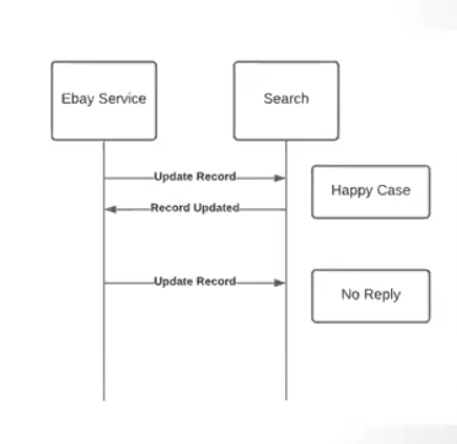
\includegraphics[scale=0.5]{images/no-update.png}
\end{center}



\vspace{\baselineskip}
If this field is \texttt{true}, we will say this means the eBay Master Service is 
in the process of updating this record, and has yet to receive a message from the eBay Search Service 
indicating it has been updated on the SearchDB. 

\vspace{\baselineskip}

We suggest created some kind of mechanism, such a CRON job, to run periodically 
to check if there are any auctions with this flag set to \texttt{true}. 
If they are \texttt{true}, send a message to the eBay Search Service asking again 
to update this record on the SearchDB table.



\subsubsection{SeqNum Field}
The \texttt{SeqNum} field has been added to the \texttt{Auction} record to help
track the order of update messages, so we know which update message each record
is waiting for. 

\vspace{\baselineskip}
If a record has \texttt{SeqNum} equal to 2, then we know it is waiting for the 
update message from the eBay Search Service with sequence number 2.




\pagebreak
\subsection{API Definition Changes}

\subsubsection{createAuction}

The \texttt{createAuction} API will need to adopt the responsibility of sending messages to the eBay Search Service's
\texttt{saveSearchableAuction} API to populate the SearchDB as new auctions are created. 
\vspace{\baselineskip}

For each new auction, \texttt{createAuction} will:

\begin{enumerate}
    \item begin a new transaction
    \item create a record in the MasterDB's Auction table
    \item set \texttt{SeqNum} to 0
    \item set \texttt{NeedUpdate} to \texttt{true}
    \item call eBay Search Service's \texttt{saveSearchableAuction} API to trigger a transaction to create 
    a new auction in the SearchDB.
    \item commit the transaction
\end{enumerate}

The eBay Master Service will then wait to receive a response from the eBay Search Service. 
If a successful response with \texttt{"success":"true"} is returned, 
\texttt{createAuction} should:

\begin{enumerate}
    \item begin a new transaction
    \item set \texttt{NeedUpdate} to \texttt{false}
    \item increment \texttt{SeqNum} by 1
    \item commit the transaction
\end{enumerate}

If no response is returned after an appropriate timeout period, \texttt{createAuction} 
should return a successful response to the \texttt{createAuction user} and do nothing.


% For any changes to the ebay master service, we need to provide:
% - Description of schema changes (not a full schema drawing)
% - Description of behavioral changes
%   - Describe new control  flow
%   - Describe transactional events
%   - Describe what happens on timeout from the search service.
% - Any additional API calls that are needed to be added to master service

\pagebreak
\subsubsection{updateAuction}

The \texttt{updateAuction} API will need to adopt the responsibility of sending messages to the eBay Search Service's
\texttt{saveSearchableAuction} API whenever an auction is updated with new information.

For each new auction update, \texttt{updateAuction} will:

\begin{enumerate}
    \item begin a new transaction
    \item update a record in the MasterDB's Auction table
    \item set \texttt{NeedUpdate} to \texttt{true}
    \item call eBay Search Service's \texttt{saveSearchableAuction} API to trigger a transaction to update an auction in the SearchDB
    \item commit the transaction
\end{enumerate}


The eBay Master Service will then wait to receive a response from the eBay Search Service. 
If a successful response with \texttt{"success":"true"} is returned, 
 \texttt{updateAuction} should:
 
 \begin{enumerate}
     \item begin a new transaction
     \item set \texttt{NeedUpdate} to \texttt{false}
     \item increment \texttt{SeqNum} by 1
     \item commit the transaction
 \end{enumerate}


 If no response is returned after an appropriate timeout period, \texttt{updateAuction} 
 should return a successful response to the \texttt{updateAuction user} and do nothing.

 
\subsubsection{findOpenAuctions}
This API from the eBay Master Service calls the eBay Search Service's \texttt{findAuctions}.
The parameters passed to the eBay Search Service's \texttt{findAuctions} API will be the same
as the parameters passed to the eBay Master Service.
\vspace{\baselineskip}

After waiting for a response, the eBay Master Service should receive a list of auction keys 
in the form of JSON.  To return the same information that is expected from the API specification 
for \texttt{findOpenAuctions}, for each auction key, the eBay Master Service will need to perform a 
\texttt{JOIN} with the MasterDB Seller table, filtering on \texttt{AuctionKey} to get \texttt{Title}, 
\texttt{Description}, \texttt{OpenDate}, \texttt{ClosingDate}, and \texttt{HighBid}.

\vspace{\baselineskip}
\vspace{\baselineskip}
\vspace{\baselineskip}
\vspace{\baselineskip}
\vspace{\baselineskip}
\vspace{\baselineskip}

NOTE: For \texttt{updateAuction} and \texttt{createAuction}, assume that sending update messages after timeouts will be handled by some mechanism that
searches for records where \texttt{NeedUpdate} is \texttt{true}.
\emph{See \hyperref[sec:needupdate]{NeedUpdate Field} for more information.}

\pagebreak
\section{Logging}

This section describes a suggested format for this service's application logs.


\begin{lstlisting}[boxpos=t,language=json,firstnumber=1]
{
    "start": <string>,
    "duration": <string>,
    "api": <string>,
    "params":
        {
            "original": {
                "auctionkey": <string>,
                "title": <string>,
                "closeDate": <string>,
                "status": <string>, 
                "category": [<string>, ...],
                "seqNum": <int> 
            }, 
            "updated": {
                "auctionkey": <string>,
                "title": <string>,
                "closeDate": <string>,
                "status": <string>,
                "category": [<string>, ...],
                "seqNum": <int> 
            }
        }
}           
\end{lstlisting}

\begin{itemize}
    \item \textbf{start} The time the service first receives the call.
    \item \textbf{duration} The amount of time it takes from when the service
        receives the call to when the service responds.
    \item \textbf{api} The name of the API that is called.
    \item \textbf{params} The original and updated data that the API changed.
        Optional data that was not changed is not included in either the
        updated or original logs.
\end{itemize}


\end{document}
